\chapter{User Manual}
\label{usermanual}
% In the user manual you should explain, step-by-step, how to reproduce the demo that you showed in the oral presentation or the results you mentioned in the previous chapters.\\ If it is necessary to install some toolchain that is already well described in the original documentation (i.e., Espressif's toolchain for ESP32 boards or the SEcube toolchain) just insert a reference to the original documentation (and remember to clearly specify which version of the original documentation must be used). There is no need to copy and paste step-by-step guides that are already well-written and available.\\The user manual must explain how to re-create what you did in the project, no matter if it is low-level code (i..e VHDL on SEcube's FPGA), high-level code (i.e., a GUI) or something more heterogeneous (i.e. a bunch of ESP32 or Raspberry Pi communicating among them and interacting with other devices).
\section{Dependencies}\label{sec:dependecies}
\begin{itemize}
  \item \texttt{Git}. In order to clone the repository with the project.
  \item \texttt{Python 3.11+}
\end{itemize}
In addition, the following Python libraries must be installed
\begin{itemize}
  \item \texttt{matplotlib}. Graph library for math visualizations
  \item \texttt{scipy}. Python library that provides mathematical instruments and algorithms
  \item \texttt{cv2}. Computer vision library, used to extract data from raw images
  \item \texttt{rawpy}. Library used to open RAW images such as CR2.
\end{itemize}

\section{Installation}\label{sec:installation}
\noindent In a shell clone the project with the following command
\begin{lstlisting}[language=bash]
  $ git clone https://github.com/doreado/camPUF.git
\end{lstlisting}

\section{Prepare the images dataset}\label{sec:preparetheimagedataset}
An images dataset could be found at \url{https://wisest.ece.wisc.edu/research-old/mobile-and-embedded-security/campuf-dataset/}.

Inside $src/auto\_testing.py$ the \texttt{img\_test\_enroll\_dir} and \texttt{img\_test\_auth\_dir} variables must be set to the folder containing the enrollment and authentication images respectively. The script searches for images automatically. The number of images used for the enrollment can be adjusted modifying the \texttt{num\_frames\_enroll} (the default value is 5). After the enrollment, the script tries to authenticate all the images in the authentication folder.

\section{Run the script}\label{sec:runthescript}
\begin{lstlisting}[language=bash]
  $ cd camPUF/src
  $ python3 auto_testing.py
\end{lstlisting}

If everything works, the output shows some information and the authentication outcomes, as shown in figure \ref{fig:resultimg}

\begin{figure}[h!]
	\vspace{0.5cm}
	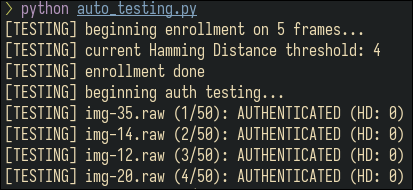
\includegraphics[width=\textwidth]{images/auto_testing_output.png}
	\caption{The output of the script has this format}
	\label{fig:resultimg}
\end{figure}
